\chapter{Theory and methods} \label{sec:theory}
\label{chapter:theory}
This section aims to briefly go over the relevant theory and specific methods that were used throughout the project work.

\section{Neural Radiance Fields}
\subsection{Vanilla NeRF}
Neural Radiance Fields\cite{nerf2020} (or NeRFs) is a method which achieves state-of-the-arts results within the field of novel view synthesis - i.e. given a set of images of a scene from different viewpoints, it can generate images from previously unseen perspective, which is essentially  

At the core of the method lies the \textit{continuous volumetric scene function}:
\begin{equation}
    (x,y,z,\theta,\phi) \rightarrow (R,G,B,\sigma)
    \label{eq:scene_function}
\end{equation}
This scene function takes a spatial location $(x,y,z)$ and a viewing direction $(\theta,\phi)$ and returns a volume density $(\sigma)$ along with a color $(R,G,B)$.

The main objective is to most effectively approximate this scene function for a specific scene. In practice, the underlying approximation is done by a fully-connected MLP (denoted $F_\Theta$). Given a set of input images, the first step is to estimate the camera poses using a photogrammetric technique such as structure-from-motion\footnote{url{https://colmap.github.io}}. Then, the idea is to essentially march rays from the estimated cameras and sample points along them (see \ref{fig:nerf_rays}). The original pixel values are used to optimize the weights of $F_\Theta$ with respect to a \textit{rendering loss} (i.e. the network is fitted such that it most faithfully reconstructs the input images).

\begin{figure}[H]
    \centering
    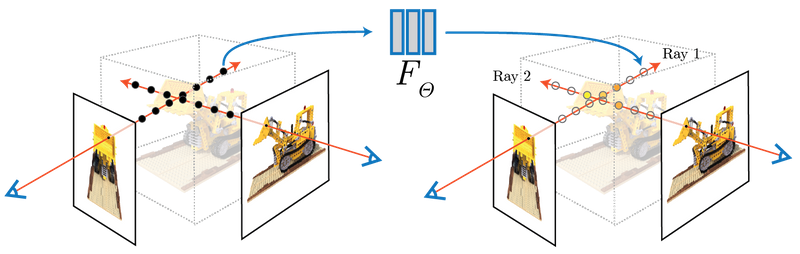
\includegraphics[width=0.85\textwidth]{figures/2_2-nerf-overview.png}
    \caption{Taken from \cite{nerf2020}. Points are sampled along the camera rays. $F_\Theta$ then returns a density ($\sigma$) and color ($(R,G,B)$) for every point. The camera rays are obtainable due to the fact that the camera poses for the input images are known.}
    \label{fig:nerf_rays}
\end{figure}

% volume rendering
An essential part of NeRFs is the aforementioned rendering loss. The idea is to take the density and color outputs from $F_\Theta$ and reduced it to a single pixel value, such that they can be compared against the ground truth (i.e. the color for the corresponding pixel in the original image data). This concept is illustrated in figure \ref{fig:nerf_render}.
\begin{figure}[H]
    \centering
    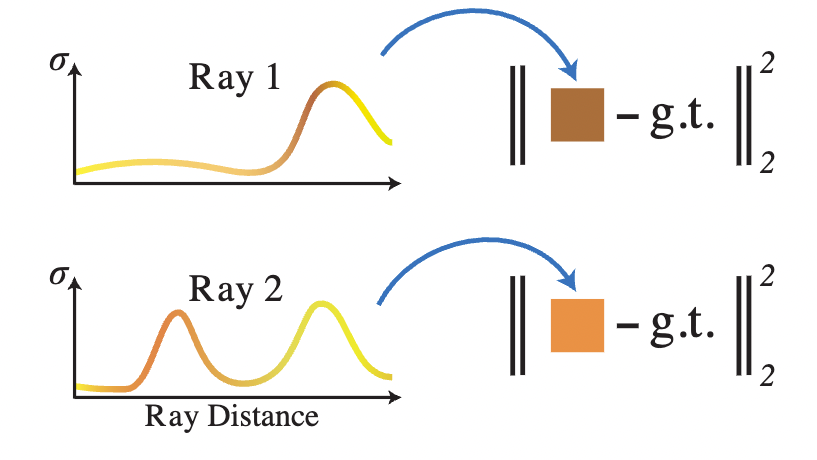
\includegraphics[width=0.8\textwidth]{figures/nerf-render.png}
    \caption{Taken from \cite{nerf2020}. Rendering loss. Using volume rendering techniques, the density and color estimates (seen on the left) are reduced to a single pixel value, which is compared against the ground truth pixel value.}
    \label{fig:nerf_render}
\end{figure}

The mechanism for reducing the ray densities and colors a single color value is inspired by classic volume rendering techniques. Formally, given the ray $\textbf{r}$ with points $\textbf{r}(t) = \textbf{o} + t \textbf{d}$, and the near/far bounds $t_n$ and $t_f$ (i.e. where the rays start, and how far the rays should extend), the continuous volume rendering formula can be stated as follows:
\begin{align}
    C(\textbf{r}) &= \int_{t_n}^{t_f} T(t) \sigma(\textbf{r}(t)) \textbf{c}(\textbf{r}(t), \textbf{d}) dt \\
    T(t) &= \exp \left( - \int_{t_n}^{t} \sigma(\textbf{r}(s)) ds \right)
    \label{eq:render-continuous}
\end{align}
The function $T(t)$ is also called the \textit{accumulated transmittance} along the ray from $t_n$ to $t$, i.e. the probability that the rays travels from $t_n$ to $t$ without hitting any other particle.

In practice, the formula is numerically estimated using quadrature. This yields the following formulation:
\begin{align}
    \hat{C}(\mathbf{r})&=\sum_{i=1}^{N} T_{i}\left(1-\exp \left(-\sigma_{i} \delta_{i}\right)\right) \mathbf{c}_{i} \\
    T_{i}&=\exp \left(-\sum_{j=1}^{i-1} \sigma_{j} \delta_{j}\right) \\
    \delta_i &= t_{i+1} - t{i}
\end{align}

The most important detail regarding the volume rendering formulae is the fact that they are trivially differentiable. This is what makes it possible to use them as loss functions for optimizing the weights of $F_\Theta$ using stochastic gradient descent.

% pos encoding
According to the authors, a big part of NeRF's success is due to the use of "Fourier features"\cite{fourer-features2020}. It turns out that passing the input coordinates $xyz\theta\phi$ through the network $F_\Theta$ resulted in poor performance when representing high-frequency variation in color and geometry, since deep neural networks are biased towards learning lower frequency functions. A solution to this problem is to map the coordinates to a higher dimensional space using some encoding function. In the original NeRF paper, the following encoding is used:
\begin{equation}
    \gamma(p) = \left(\sin(2^0 \phi p), \cos(2^0\pi p), ..., \sin(2^{L-1} \phi p), \cos(2^{L-1}\pi p) \right)
    \label{eq:nerf_enc}
\end{equation}

Equation \ref{eq:nerf_enc} maps an input coordinate from $\mathbb{R}$ to $\mathbb{R}^{2L}$, and is actually quite similar to how the positional encoding is performed in \cite{vaswani2017} (although it is used for a different purpose).

% nerf architecture
To ensure volumetric consistency (e.g. the density $\sigma$ at point $[x,y,z]$ is the same no matter the viewing direction $[\theta,\phi]$), the network $F_\Theta$ is regularized by returning $\sigma$ before adding the viewing direction as a network input. As such, the density is now estimated by a spatial density function (i.e. depends only on $[x,y,z]$), whereas the the color $(R,G,B)$ is estimated by a spatiodirectional function (i.e. depends on $[x,y,z,\theta,\phi]$. The architecture containing this constraint is shown in figure \ref{fig:nerf-arch}
\begin{figure}[H]
    \centering
    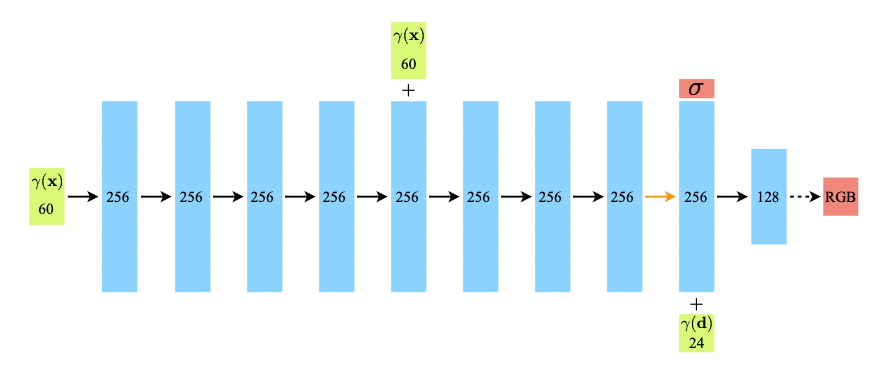
\includegraphics[width=0.8\textwidth]{figures/nerf-arch.png}
    \caption{Taken from \cite{nerf2020}. Architecture of $F_\Theta$. Input vectors are green. Hidden layers are blue. All layers are fully-connected layers. Black arrows indicate ReLU, orange arrows indicate no activation, dashed arrows indicate sigmoid activation. "+" indicates vector concatenation. \textbf{x} denotes the 3D position, \textbf{d} denotes the viewing direction.}
    \label{fig:nerf-arch}
\end{figure}


% ablation study
An ablation study was performed in the NeRF paper in order to determine the effectiveness of the different components. This can be seen in figure \ref{fig:nerf-ablation}.
\begin{figure}[H]
    \centering
    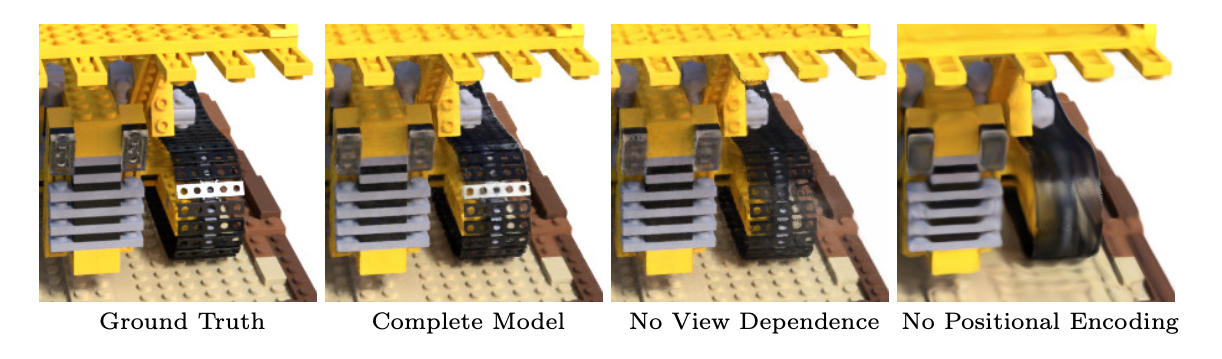
\includegraphics[width=0.85\textwidth]{figures/nerf-ablation.png}
    \caption{Taken from \cite{nerf2020}. NeRF ablation study. "View dependence" refers to the notion of incorporating viewing directions (i.e. camera ray directions) in $F_\Theta$. "Positional encoding" refers to the notion of applying the $\sin/\cos$-encoding to input coordinates. Removing view dependence prevents the model from recreating the specular reflection on the bulldozer tread. Removing the positional encoding inhibits the model in terms of representing high frequency geometry and colors, resulting in an oversmoothed image.}
    \label{fig:nerf-ablation}
\end{figure}


% instant-ngp
Recently, a huge leap was made in optimizing the efficiency of NeRFs. The training time for a vanilla NeRF is in the range of 12-24 hours - with the work done in \cite{mueller2022}, the training time is in the order of minutes instead. The main idea of the paper is the introduction of "multiresolution hash encoding", which essentially works by trilinearly interpolating multiple discrete 3D grids of trainable embeddings.

In short, the authors of \cite{mueller2022} largely attribute the speed gains to using a smaller MLP (smaller in both width/depth). This downsize is made possible by the fact that the $\sin/\cos$-based positional encoding is replaced with the more powerful multiresolution hash encoder. Another contributing factor is the fact that highly efficient CUDA kernels were developed specifically for the project.

\subsection{NeRF disentanglement}
Recently, a framework for volumetrically disentangling objects from the background of NeRF scenes was proposed in \cite{benaim2022}. 

In a standard NeRF setup, a dataset of images (and camera poses) is given. Now, a set of 2D masks for the object of interest should also be provided. The masks are used to apply a \textit{masked} rendering loss. An illustration of this can be seen in figure \ref{fig:disent-training}.
\begin{figure}[H]
    \centering
    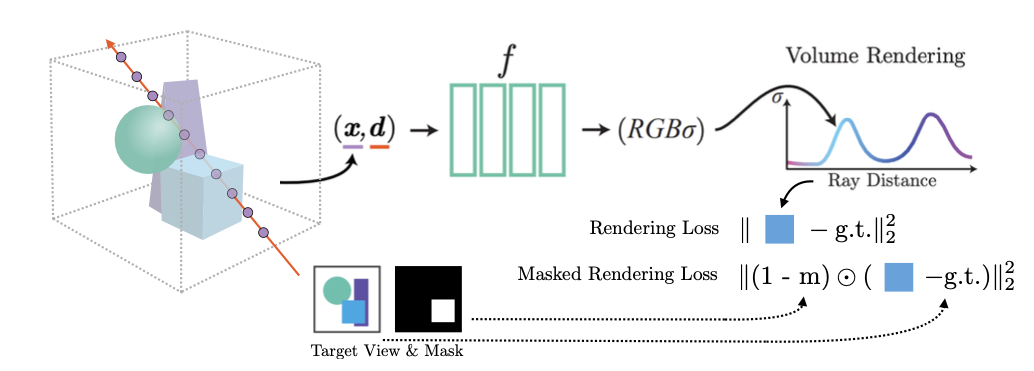
\includegraphics[width=0.8\textwidth]{figures/disent-training.png}
    \caption{Taken from \cite{benaim2022}. Masked rendering loss.}
    \label{fig:disent-training}
\end{figure}

Thus, two NeRFs are trained in total - the full scene (i.e. regular rendering loss), and the background scene (i.e. masked rendering loss). The idea is then to obtain the foreground scene by subtracting the background scene from the full scene. This is performed according to the following formulae:
\begin{align}
    c_{r}^{fg} &= \sum_{i=1}^N w_{fg}^{i} \cdot c_{fg}^{i} \\
    w_{fg}^{i} &= w_{full}^{i} - w_{bg}^{i} \\
    c_{fg}^{i} &= c_{full}^{i} - c_{bg}^{i}
\end{align}
In other words, the weights and colors are subtracted from each other separately before being multiplied together to obtain the foreground scene.

An excerpt of the results reported in \cite{benaim2022} can be seen in figure \ref{fig:disent-results}.
\begin{figure}[H]
    \centering
    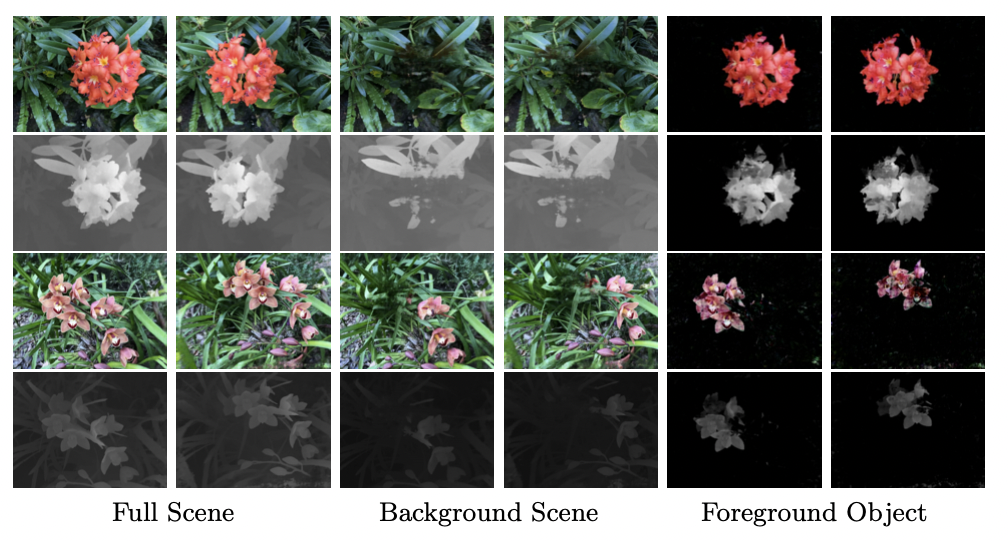
\includegraphics[width=1.0\textwidth]{figures/disent-results.png}
    \caption{Taken from \cite{benaim2022}. Example results for foreground object disentanglement.}
    \label{fig:disent-results}
\end{figure}


The work also shows examples of how disentangled foreground objects can be re-inserted into the background scenes after applying some type of transformation. This can be seen in figure \ref{fig:tv-example}.
\begin{figure}[H]
    \centering
    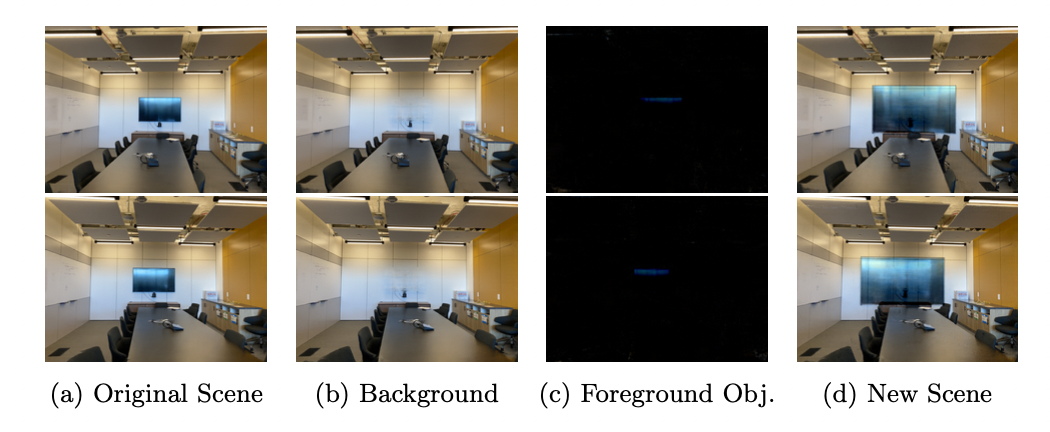
\includegraphics[width=0.85\textwidth]{figures/tv-example.png}
    \caption{Taken from \cite{benaim2022}. Re-insertion of a transformed foreground object. The TV has been scaled before being re-inserted into the original scene, and still appears to respect illumination. Thus, the scene itself still retains its photo-realistic appearance.}
    \label{fig:tv-example}
\end{figure}


\subsection{NeRF manipulation}
\label{sec:nerf-manipulation}
The goal is to be able to scale, rotate and transform the objects freely in 3D space. As such, additional techniques for transforming disentangled foreground objects are needed. The main idea behind the approach taken for NeRF manipulation in this project is to apply an affine transformation to the camera rays before sending them through NeRF.

Let's start with translation. Let the vector $\textbf{t} = [\delta_x, \delta_y, \delta_z]$ denote the desired translation. The idea is to add the translation vector to the camera rays. An example translation can be seen in figure \ref{fig:manip-trans}:
\begin{figure}[H]
    \centering
    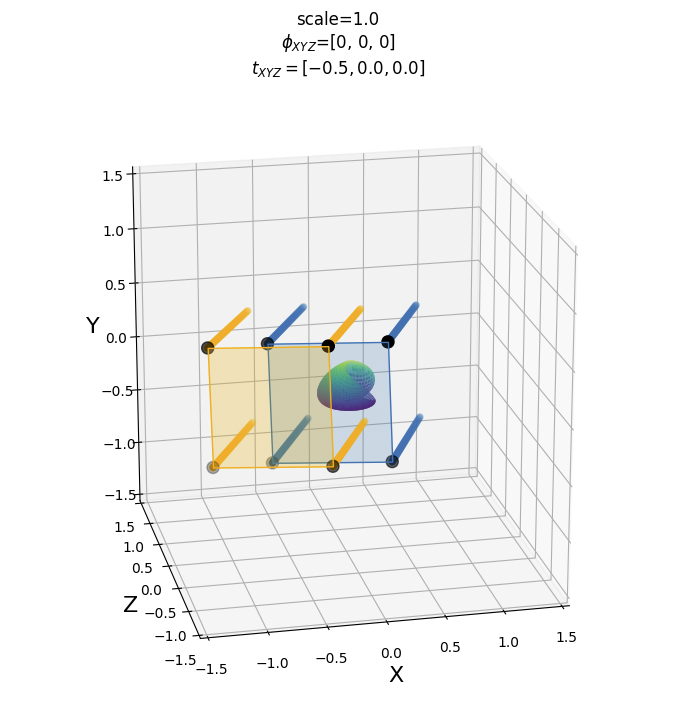
\includegraphics[width=0.8\textwidth]{figures/manip-trans.png}
    \caption{Translation along the x-axis. The square polygon faces denotes a camera image, and the lines denote the camera rays. Blue denotes unmodified camera, orange denotes modified camera. This has the effect of moving the object to the right (i.e. further along in the x-direction).}
    \label{fig:manip-trans}
\end{figure}


Now, for rotation, the rays are going to be multiplied with a $3\times3$ rotation matrix, which is defined as follows (where $[\alpha,\beta,\gamma] = [x,y,z]$-rotation):
\begin{equation}
    \textbf{R} = R_{z}(\gamma) R_{y}(\beta) R_{x}(\alpha) = {\left[\begin{array}{ccc}
    \cos \gamma & -\sin \gamma & 0 \\
    \sin \gamma & \cos \gamma & 0 \\
    0 & 0 & 1
    \end{array}\right]\left[\begin{array}{ccc}
    \cos \beta & 0 & \sin \beta \\
    0 & 1 & 0 \\
    -\sin \beta & 0 & \cos \beta
    \end{array}\right]\left[\begin{array}{ccc}
    1 & 0 & 0 \\
    0 & \cos \alpha & -\sin \alpha \\
    0 & \sin \alpha & \cos \alpha
    \end{array}\right] }
\end{equation}
A centre of rotation is also defined using the vector $\textbf{c} = [c_x, c_y, c_z]$. By default, let $\textbf{c} = [0,0,0]$ (i.e. rotation about the origin). An example rotation can be seen in figure \ref{fig:manip-rotation}.
\begin{figure}[H]
    \centering
    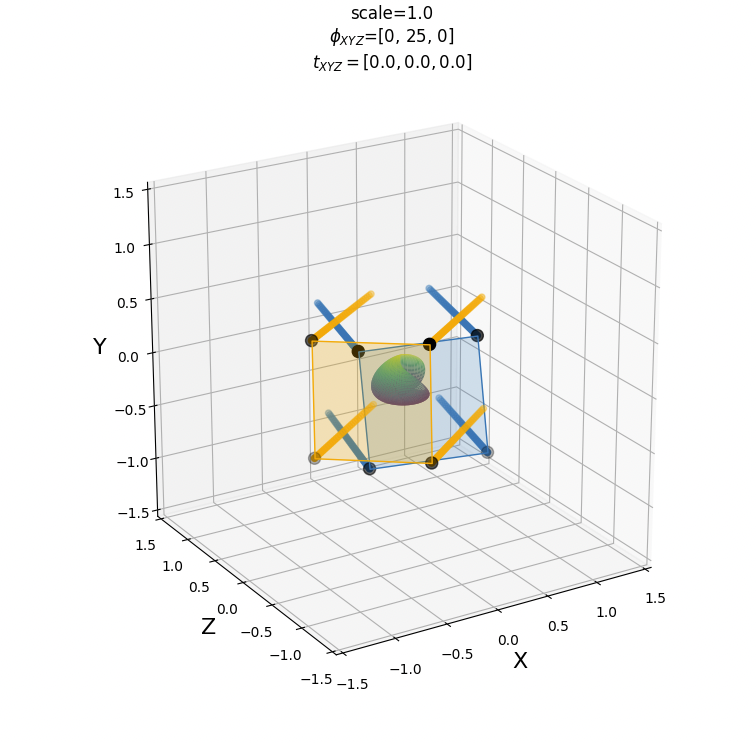
\includegraphics[width=0.8\textwidth]{figures/manip-rotation.png}
    \caption{Rotation around the z-axis. The square polygon faces denotes a camera image, and the lines denote the camera rays. Blue denotes unmodified camera, yellow denotes modified camera. This has the effect of rotating the object 25 degrees counter-clockwise about y.}
    \label{fig:manip-rotation}
\end{figure}

Now it's time to define operations for scaling. Let $s$ denote a scalar value which will control scale. Then let $\textbf{S} = \begin{bmatrix}\frac{1}{s} & 0 & 0 \\ 0 & \frac{1}{s} & 0 \\ 0 & 0 & 1\end{bmatrix}$ be a scaling matrix which is designed to scale the $x$ and $y$ components of our ray origins (as such, the operation leaves ray directions intact).

Before applying the scaling matrix, the rays must first be aligned with the unit vector $[0,0,1]$. To achieve this, we need to determine the matrix $\textbf{A}$ which rotates the unit vector $[0,0,1]$ such that it is aligned with the ray direction vector. While there likely exists a closed form solution to this, it was easier to just use a Kabsch algorithm (which exists in scipy). Thus, the scaling operation is performed by the chain of matrix products $\textbf{A}^{-1} \textbf{S} \textbf{A}$, where $\textbf{A} = \text{align}([0,0,1], \textbf{d})$. An example of the scaling operation can be seen in figure \ref{fig:manip-scale}.
\begin{figure}[H]
    \centering
    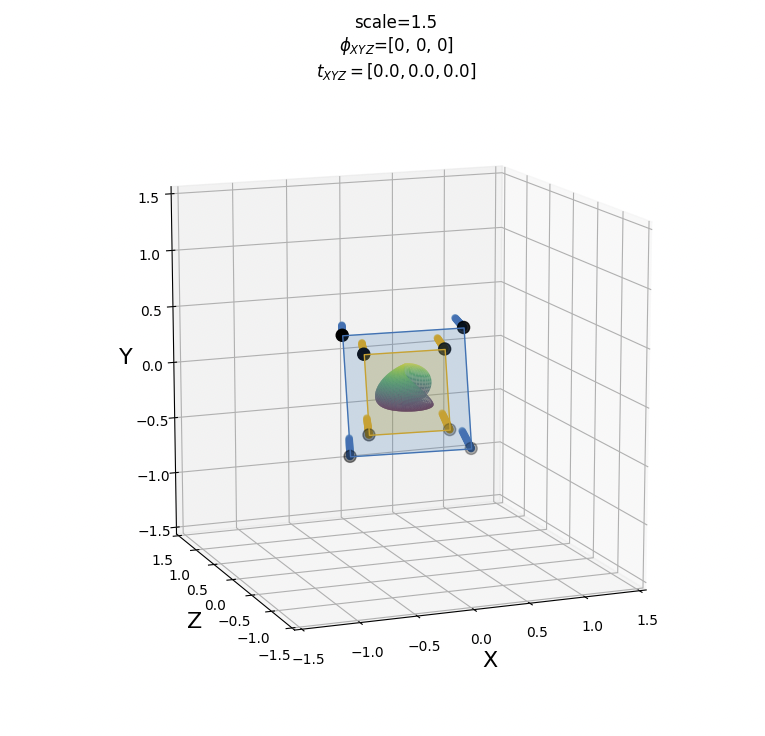
\includegraphics[width=0.8\textwidth]{figures/manip-scale.png}
    \caption{Scaling operation. The square polygon faces denotes a camera image, and the lines denote the camera rays. Blue denotes unmodified camera, yellow denotes modified camera. By transforming the ray origins such that they are closer together, the object effectively appears larger.}
    \label{fig:manip-scale}
\end{figure}

Recall the ray definition $\textbf{r}(t) = \textbf{o} + t \textbf{d}$. Now, combining translation, rotation and scaling, the full transformed ray definition can be stated as follows:
\begin{align}
    \hat{\textbf{r}}(t) &= ((\textbf{o}-\textbf{c}) \textbf{A}^{-1} \textbf{S} \textbf{A})\textbf{R} + t \left((\textbf{d} - \textbf{c})\textbf{R} + \textbf{c}\right) + \textbf{c} + \textbf{t}
\end{align}

An example which performs all transformations at once can be seen in figure \ref{fig:manip-comb}.
\begin{figure}[H]
    \centering
    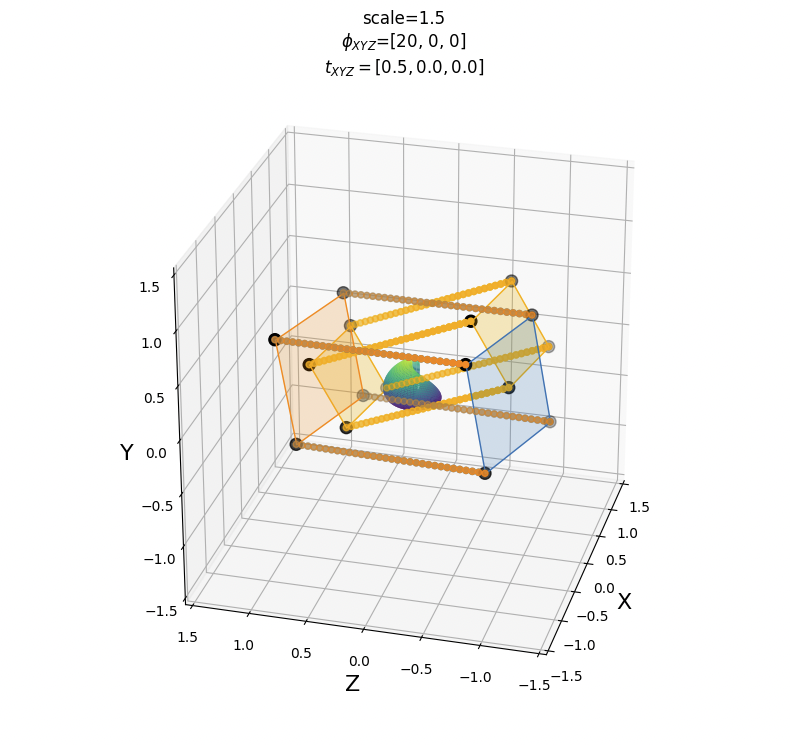
\includegraphics[width=0.7\textwidth]{figures/manip-comb.png}
    \caption{Combined transformation. To illustrate the consistency of the transformations for different views, an additional orange camera has been inserted directly opposite of the existing blue camera. The modified cameras are yellow.}
    \label{fig:manip-comb}
\end{figure}

There is an additional important detail about re-inserting transformed disentangled objects. The transformation must also be applied to the background scene before performing volumetric subtraction. In order words, given the full scene $F_{full}$ and the background scene $F_{background}$, let $G_{full}$ denote the transformed full scene, and $G_{background}$ the transformed background scene. Now, the volumetric re-insertion is formulated as follows:
\begin{equation}
    (G_{full} - G_{background}) + F_{background}
\end{equation}

Recall that $\textbf{c} = [0,0,0]$, which means that the rotation still revolves about the origin. If the transformation should be object-centric, it would require that the centre point of the object is known (or at least estimated). A potential mechanism for this would be to use the marching cubes algorithm (see figure \ref{fig:marching-cubes}) to produce a mesh for the foreground object, which can then be used to determine the voxel centroid (i.e. the "centre of mass" of the mesh).
\begin{figure}[H]
    \centering
    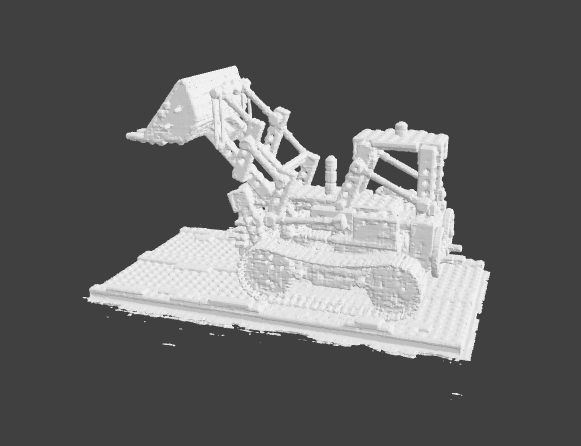
\includegraphics[width=0.7\textwidth]{figures/marching-cubes.png}
    \caption{Taken from \cite{nerf2020}. Marching cubes produces a mesh for the NeRF bulldozer scene. The mesh can be used to calculate a centre point of the foreground object, which can be used to perform object-centric transformations (e.g. rotation about the object itself)}
    \label{fig:marching-cubes}
\end{figure}

\section{Semantic guidance}
\subsection{CLIP}
Recent advances have been made in the field of vision-language modeling - a very notable one being OpenAI's CLIP\cite{radford2021}.

At its core, it contains an image encoder and a text encoder. The image encoder is based on either a ResNet\cite{resnet-paper} or a Vision Transformer\cite{vit-paper} architecture. The text encoder is based on a Transformer\cite{vaswani2017} architecture. The encoders are configured to produce vectors of the same dimensionality.

A fundamental concept in CLIP is the contrastive pre-training process. Given a dataset of image-text pairs, the encoders are jointly optimized such that they produce vectors that align for the matching image-text pairs, and don't align for the non-matching image-text pairs. In other words, it seeks to maximize the cosine similarity of the embeddings for matching pairs.

\begin{figure}[H]
    \centering
    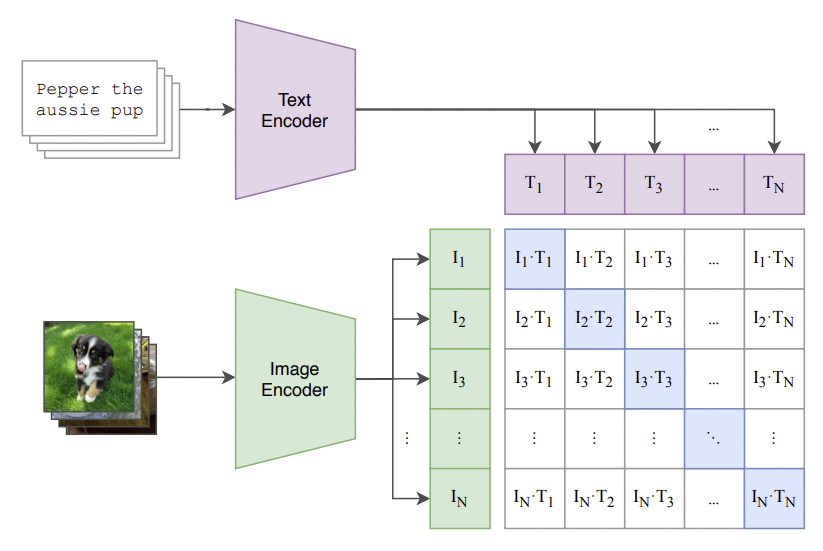
\includegraphics[width=0.7\textwidth]{figures/clip-contrast.png}
    \caption{Taken from \cite{radford2021}. CLIP contrastive pre-training}
    \label{fig:clip-contrast}
\end{figure}

The contrastive pre-training is performed in batches of size $N$. As such, there are $N^2$ pairs to consider for every batch - of which only $N$ pairs are matches. This is illustrated in figure \ref{fig:clip-contrast}, with the diagonal of the matrix indicating the matching pairs for which the similarity should be maximized.

A benefit of pre-training models in this contrastive fashion is the fact that no dataset labels are required. This makes it easier to gather huge datasets by scraping the internet, where a lot of text-image pairs can be found naturally (e.g. Instagram, reddit, etc.). However, despite being trained on a massive dataset, there might still be "holes" in CLIP's representation space. For instance, it might not appropriately embed an image due to lighting conditions, image noise, and other visual artifacts. As such, it might be important to heavily augment or somehow regularize the signals obtained from CLIP.

After pre-training, CLIP is capable of embedding instances of different modalities (i.e. text and images) into the same space. This has led to a lot of additional research involving its capabilities as a zero-shot image classifier (zero-shot meaning "not trained for the specific task").
\begin{figure}[H]
    \centering
    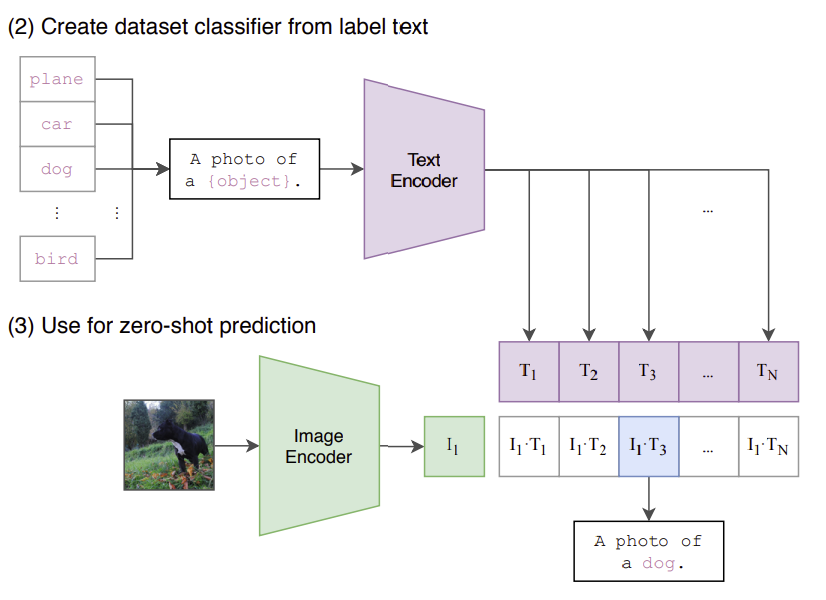
\includegraphics[width=0.7\textwidth]{figures/clip-zeroshot.png}
    \caption{Taken from \cite{radford2021}. CLIP zero-shot prediction}
    \label{fig:clip-zeroshot}
\end{figure}

Figure \ref{fig:clip-zeroshot} shows how a zero-shot classifier can be made. The main idea is to produce a set of text prompts based on the classes that are present in the dataset. Then, all the text prompts can be encoded as CLIP vectors. Now, given a new input image, the classifier simply encodes the image to obtain a CLIP vector, and calculates the cosine similarities in order to determine which class yields the highest similarity, which will be the predicted class.

\subsection{Shattered gradients}
\label{sec:shattered-gradients}
The shattered gradients problem occurs when working with deep neural network architectures (such as the ones used in CLIP). The work done in \cite{balduzzi2017} shows that the correlation between gradients in standard feedforward networks decays exponentially with network depth, which ultimately results in gradients that resemble white noise. On the other hand, the gradients in networks that implement skip-connections decay sublinearly, which makes them more resilient to gradient shattering.


In \cite{balduzzi2017}, an example neural network can be constructed. It maps from $\mathbb{R} \rightarrow \mathbb{R}$ (i.e. scalars to scalar), and contains $N=200$ rectifier units per hidden layer. The gradient with respect to the input $x_i$ is computed for 256 values of $x_i \in [-2,2]$. This has been done for multiple network architectures (including ResNet, which has skip-connections). The results can be seen in figure \ref{fig:balduzzi-gradients}.
\begin{figure}[H]
    \centering
    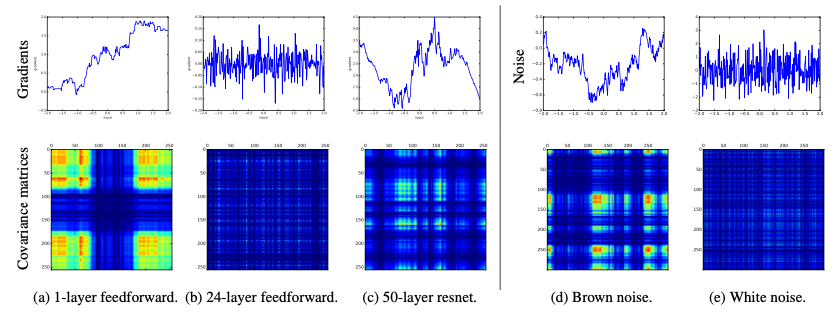
\includegraphics[width=0.90\textwidth]{figures/balduzzi-gradients.png}
    \caption{Taken from \cite{balduzzi2017}. Comparison between noise and gradients of rectifier nets with 200 neurons per hidden layer.}
    \label{fig:balduzzi-gradients}
\end{figure}

Figure \ref{fig:balduzzi-gradients} shows that the gradients (and covariance matrices) resemble white noise for the deep feedforward network, and brown noise for the ResNet. This is explored even further in \cite{balduzzi2017}, where the phenomenon is illustrated by plotting the autocorrelation function (ACF) for noise compared to the gradients from different network architectures at various depths ranging between $[2,50]$.
\begin{figure}[H]
    \centering
    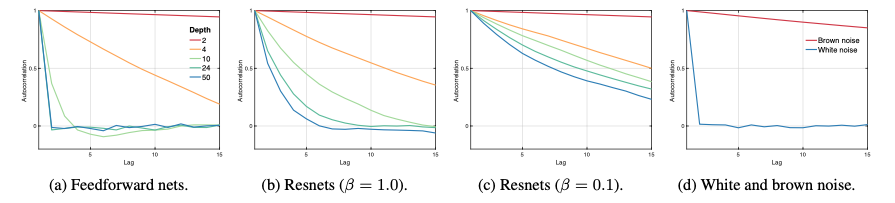
\includegraphics[width=0.95\textwidth]{figures/balduzzi-acf.png}
    \caption{Taken from \cite{balduzzi2017}. Autocorrelation functions (ACF) for the gradients from various network architectures compared to white and brown noise.}
    \label{fig:balduzzi-acf}
\end{figure}

Figure \ref{fig:balduzzi-acf} illustrates the impact of network depth on gradient noise. For standard feedforward nets, the gradient ACF already becomes similar to the ACF of white noise at a depth of 10. For ResNets, the gradient ACF seems to be more similar to the ACF of brown noise (depending on the rescaling parameter $\beta$).


\section{Full pipeline}
Combining the methods from the previous sections yields the full pipeline for semantically guided volumetric object manipulation. Given a differentiable renderer (in our case NeRF) which supports a set of transformation parameters \textbf{s}, the goal is to determine the most optimal parameter values with respect to a given text prompt. The similarity will be driven by CLIP. A diagram of the pipeline can be seen in figure \ref{fig:full-pipeline}.
\begin{figure}[H]
    \centering
    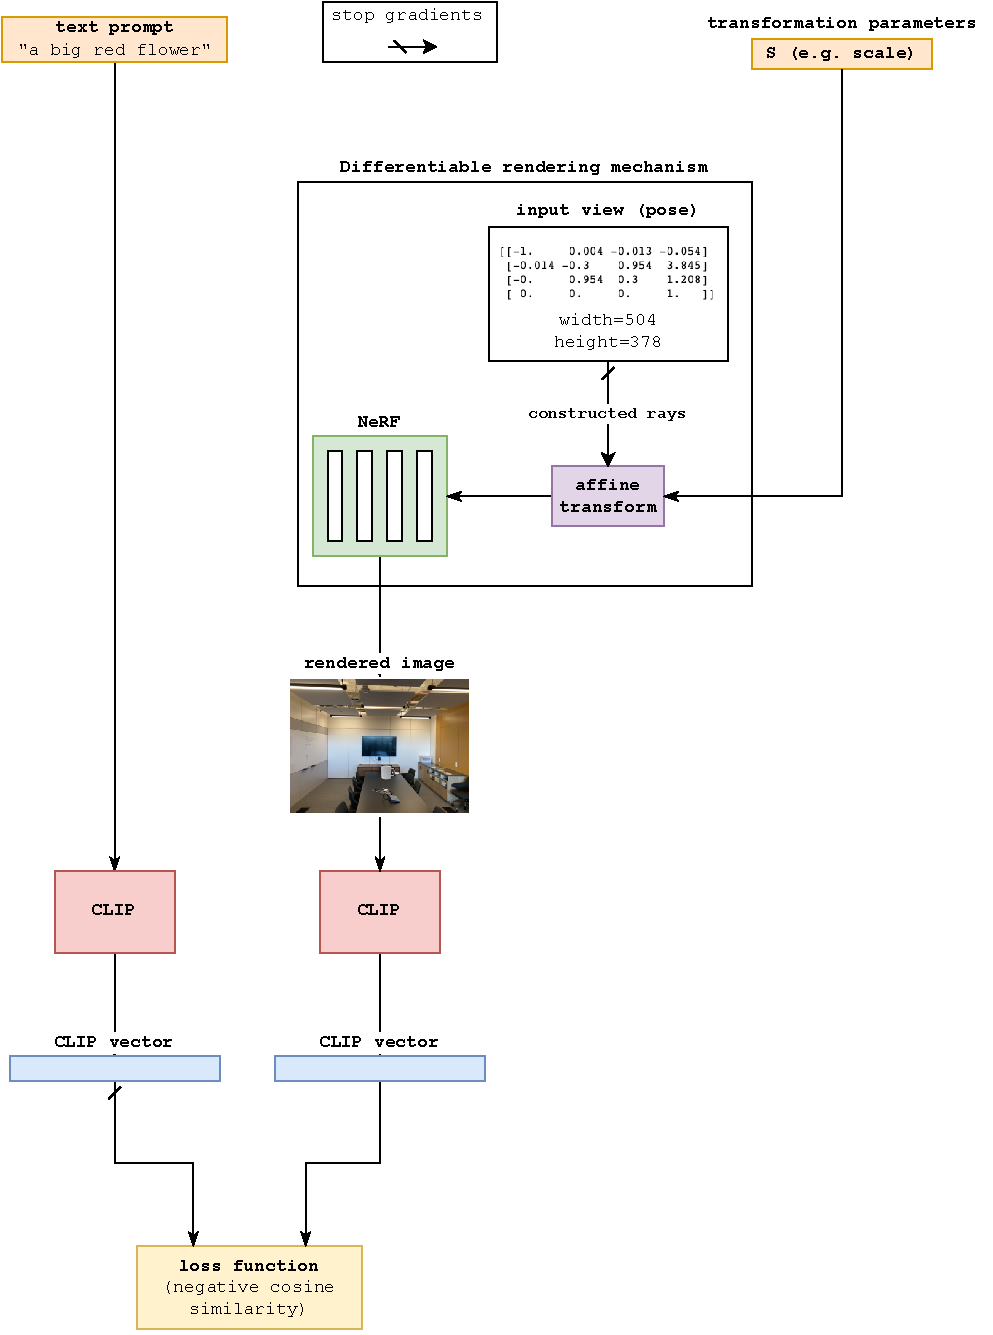
\includegraphics[width=1.0\textwidth]{figures/full-pipeline.pdf}
    \caption{Diagram of the full pipeline for semantically guided volumetric object manipulation.}
    \label{fig:full-pipeline}
\end{figure}
